\documentclass[12pt,a4paper,oneside]{article}
\usepackage[spanish,es-noshorthands]{babel}
\usepackage{tikz, pgfplots, geometry, graphicx, wrapfig, tipa, circuitikz} % Entornos graficos
\usepackage{amssymb, amsmath, float, mathpazo, textcomp, gensymb, mathtools,mathrsfs} % Matematica/Simbolos
\usepackage{multicol, multirow, xcolor, colortbl}
\usepackage{lastpage, bookmark, authblk}
\usepackage{subcaption}
\usepackage{array}

% Varios
\usepackage[label=corner]{karnaugh-map}
\usepackage{threeparttable}
\usepackage{ulem, lipsum}
\usepackage{adjustbox}
\usepackage{listings}
\usepackage{fancyhdr}
\usepackage{capt-of}
\usepackage{caption}
\usepackage{cancel}
\usepackage{makecell} % Para hacer saltos de linea en tablas
\usepackage[utf8]{inputenc} % Required for inputting international characters
\usepackage[T1]{fontenc} % Output font encoding for international characters

% Librerias extra de Tikz
\pgfplotsset{compat=1.7} % !!VERSION PGF¡¡
\usetikzlibrary{patterns}
\usetikzlibrary{positioning}
\usetikzlibrary{arrows}
\usetikzlibrary{calc}
\usetikzlibrary{fpu}
\usepackage{longtable}

\definecolor{vgreen}{RGB}{104,180,104}
\definecolor{vblue}{RGB}{49,49,255}
\definecolor{vorange}{RGB}{255,143,102}
\definecolor{codegreen}{rgb}{0,0.6,0}
\definecolor{codegray}{rgb}{0.5,0.5,0.5}
\definecolor{codepurple}{rgb}{0.58,0,0.82}
\definecolor{backcolour}{rgb}{0.95,0.95,0.92}
\definecolor{mlgb}{RGB}{100,224,238}
\definecolor{mdrd}{RGB}{160,24,82}
\definecolor{mdblu}{RGB}{20,91,112}
\definecolor{mblk}{RGB}{35,35,35}


\usepackage[scr=esstix,cal=boondox]{mathalfa}
\makeatletter
\usepackage[spanish,es-noshorthands]{babel}
\usepackage{tikz, pgfplots, geometry, graphicx, wrapfig, tipa, circuitikz} % Entornos graficos
\usepackage{amssymb, amsmath, float, mathpazo, textcomp, gensymb, mathtools,mathrsfs} % Matematica/Simbolos
\usepackage{multicol, multirow, xcolor, colortbl}
\usepackage{lastpage, bookmark, authblk}
\usepackage{subcaption}
\usepackage{array}

% Varios
\usepackage[label=corner]{karnaugh-map}
\usepackage{threeparttable}
\usepackage{ulem, lipsum}
\usepackage{adjustbox}
\usepackage{listings}
\usepackage{fancyhdr}
\usepackage{capt-of}
\usepackage{caption}
\usepackage{cancel}
\usepackage{makecell} % Para hacer saltos de linea en tablas
\usepackage[utf8]{inputenc} % Required for inputting international characters
\usepackage[T1]{fontenc} % Output font encoding for international characters

% Librerias extra de Tikz
\pgfplotsset{compat=1.7} % !!VERSION PGF¡¡
\usetikzlibrary{patterns}
\usetikzlibrary{positioning}
\usetikzlibrary{arrows}
\usetikzlibrary{calc}
\usetikzlibrary{fpu}
\usepackage{longtable}

\definecolor{vgreen}{RGB}{104,180,104}
\definecolor{vblue}{RGB}{49,49,255}
\definecolor{vorange}{RGB}{255,143,102}
\definecolor{codegreen}{rgb}{0,0.6,0}
\definecolor{codegray}{rgb}{0.5,0.5,0.5}
\definecolor{codepurple}{rgb}{0.58,0,0.82}
\definecolor{backcolour}{rgb}{0.95,0.95,0.92}
\definecolor{mlgb}{RGB}{100,224,238}
\definecolor{mdrd}{RGB}{160,24,82}
\definecolor{mdblu}{RGB}{20,91,112}
\definecolor{mblk}{RGB}{35,35,35}


\usepackage[scr=esstix,cal=boondox]{mathalfa}

%Caratula
\newcommand{\subtitledoc}[1]{\newcommand{\@subtitledoc}{#1}}
\newcommand{\instituto}[1]{\newcommand{\@instituto}{#1}}
\newcommand{\carrera}[1]{\newcommand{\@carrera}{#1}}
\newcommand{\professor}[1]{\newcommand{\@professor}{#1}}
\newcommand{\catedra}[1]{\newcommand{\@catedra}{#1}}
\newcommand{\curso}[1]{\newcommand{\@curso}{#1}}
\newcommand{\legajo}[1]{\newcommand{\@legajo}{#1}}
\newcommand{\footerauthor}[1]{\newcommand{\@footerauthor}{#1}}
\newcommand{\footerlegajo}[1]{\newcommand{\@footerlegajo}{#1}}
\newcommand{\footercatedra}[1]{\newcommand{\@footercatedra}{#1}}

%Indice
\newcommand{\unsection}[1]{\addcontentsline{toc}{section}{#1}\section*{#1}}
\newcommand{\unsubsection}[1]{\addcontentsline{toc}{subsection}{#1}\subsection*{#1}}
\newcommand{\unsubsubsection}[1]{\addcontentsline{toc}{subsubsection}{#1}\subsubsection*{#1}}

%Custom
\newcommand{\longdiv}{\smash{\mkern-0.43mu\vstretch{1.31}{\hstretch{.7}{)}}\mkern-5.2mu\vstretch{1.31}{\hstretch{.7}{)}}}}
\newcommand{\lrah}{\hspace{0.25cm} \Longrightarrow \hspace{0.25cm}}
\newcommand{\llah}[1]{\hspace{0.25cm} \Longleftarrow \hspace{0.25cm}}
\newcommand{\llrah}[1]{\hspace{0.25cm} \Longleftrightarrow \hspace{0.25cm}}
\newcommand{\Real}[1]{\mathbb{R}{e}\{#1\}}
\newcommand{\Imag}[1]{\mathbb{I}{m}\{#1\}}
\newcommand{\arc}[1]{{%
    \setbox9=\hbox{#1}%
    \ooalign{\resizebox{\wd9}{\height}{\texttoptiebar{\phantom{A}}}\cr#1}}}


%Configuracion de hoja (margenes y tamaño)
\geometry{a4paper,margin=1in}
\setlength\headheight{28pt}





%Metadata para pdf
%\hypersetup{
%    pdftitle={\@title},
%    pdfsubject={\@catedra\ - \@subtitledoc},
%    pdfauthor={\@author\ - \@legajo\ - \@curso},
%    pdfkeywords={\@title\ \@catedra\ \@subtitledoc\ \@author\ \@legajo\ \@curso}
%}






%formato de encabezado y pie para todas las paginas.
\fancyhead[L]{
    \begin{minipage}[b]{7.5mm}
        
\includegraphics[width=7mm]{Imagenes/logo-utn.png}
    \end{minipage}
    \begin{minipage}[b]{100mm}
        \textbf{Alumnos: }\@footerauthor \\
        \textbf{Legajos: }\@footerlegajo
    \end{minipage}
}
\fancyhead[R]{
    \textbf{Curso:} \@curso \textbf{ - Año:} \the\year\\%/\twodigits\the\month/\twodigits\the\day\\
    \textbf{Cátedra:} \@catedra
}
\fancyfoot[C]{} %eliminar antiguo numero de pagina
\fancyfoot[R]{Página \thepage\ de \pageref{LastPage}}
\renewcommand{\headrulewidth}{0.5pt}
\renewcommand{\footrulewidth}{0.5pt}
\pagestyle{fancy}
\addto\captionsspanish{%
	\renewcommand{\contentsname}%
	{CONTENIDO}%
}

\renewcommand{\maketitle}{%
    \newpage
    \thispagestyle{empty}
    
    \begin{center}

    \textsc{\LARGE \@instituto}\\[0.5cm] 
    \textsc{\Large \@carrera}\\[1.5cm] 
    
\includegraphics[width=0.30\textwidth]{Imagenes/logo-utn.png} \par
    \vspace{0.9cm}
    
    \textsc{\large \@catedra}\\[0.85cm]
    \headrule \vspace{0.25cm}
    {\huge\bfseries \@title}\\[0.4cm]
    \textsc{\Large \@subtitledoc}\\[0.25cm]
    \headrule \vspace{0.25cm}
    
    \end{center}

    \vspace{2cm}

    {\noindent
    \begin{minipage}[t]{.2\textwidth}
        \raggedright
        \textbf{DOCENTES} \par
        \bigskip \bigskip
        \smallskip
        \textbf{CÁTEDRA} \par
        \textbf{CURSO} \par
        \medskip
        \textbf{ALUMNOS} \par
        \end{minipage}%
        \begin{minipage}[t]{.05\textwidth}
        \raggedright
        \textbf{:} \par
        \bigskip \bigskip
        \smallskip
        \textbf{:} \par
        \textbf{:} \par
        \medskip
        \textbf{:} \par
    \end{minipage}%
    \begin{minipage}[t]{.55\textwidth}
        \raggedright
        \@professor \par
        \@catedra \par
        \@curso \par
        \medskip 
        \@author \par
    \end{minipage}%
    \begin{minipage}[t]{.15\textwidth}
        \raggedright
        ~\\
        ~\\
        ~\\
        ~\\
         \bigskip \bigskip
        \@legajo \par
    \end{minipage}
    }
    \vfill
    \begin{center}
        \textbf{CÓRDOBA, ARGENTINA} \par
        \textbf{\@date}
    \end{center}
    \newpage
}

\makeatother


\instituto{Universidad Tecnológica Nacional\\Facultad Regional Córdoba}
\carrera{Ingeniería Electrónica}
\title{Análisis de señales y Mediciones básicas con Osciloscopios}
\subtitledoc{Trabajo Práctico de Laboratorio Nº 2}
\professor{
   JTP Ing. Luis Alberto Guanuco, \par
   Ing. Carlos Centeno, \par
   Ing. Martín Salamero.
}
\catedra{Medidas Electrónicas I}
\curso{4R1}
\author{
    Robertson, Máximo. \par 
    Musso, Lucas.  \par 
    Arenas, Nicolás. \par 
    Palacios, Alexandro. \par 
}
\legajo{
    89712 \par 
    91934 \par 
    86607 \par 
    91454 \par
}
\footerauthor{
Robertson, Musso, Arenas, Palacios.
}
\footerlegajo{  
    89712, 91934, 86607, 91454.
}


\begin{document}
\maketitle

\tableofcontents
\newpage


\section{Introducción}
%En este segundo trabajo práctico de laboratorio de la materia Medidas Electrónicas I, se analizarán y medirán señales en el dominio del tiempo con osciloscopios tanto analógicos como digitales. En esta oportunidad, se realizarán múltiples experimentos donde se verán de manera práctica los conceptos aprendidos en clase, con el objetivo de adquirir experiencia en el uso de osciloscopios para efectuar el análisis y la medición de algunos parámetros en distintos tipos de formas de ondas.

\subsection{Roles de los Integrantes}

La división de las tareas dentro de nuestro grupo en este trabajo será la siguiente: 

\begin{table}[h!]
    \centering
    \begin{tabular}{|c|c|}
    \hline
        Alumno & Rol \\
    \hline
        Musso, Lucas & Coordinador \\ 
        Arenas, Nicolás & Operador 1 \\
        Palacios, Alexandro & Operador 2 \\
        Robertson, Máximo & Documentación \\
    \hline
        \end{tabular}
        \def\tablename{Tabla} 
        \caption{Tabla de asignación de roles para cada integrante}
        \label{tab:roles}
\end{table}

La fecha de entrega estipulada en el cronograma entregado a los docentes para este trabajo práctico es del \textbf{\textit{16 de mayo del 2024}}.

Y la fecha en que el equipo rendirá el coloquio oral será también el día \textbf{\textit{16 de mayo del 2024}}.



\subsection{Grilla de Evaluación}

\begin{table}[H]
    \centering
    \scalebox{0.895}{
    \begin{tabular}{|c|p{6.5cm}|c|c|c|c|c|}
    \hline
        \multirow{2}{*}{ID} & \multirow{2}{*}{Criterio de Evaluación} & \multicolumn{4}{c|}{\%Obt.} & \multirow{2}{*}{\%max} \\ 
        \cline{3-6}
        ~ & ~ & ECG & EO1 & EO2 & ED & ~ \\ \hline
        CEval 1 & Identifica los datos necesarios para determinar especificaciones de los instrumentos disponibles & ~ & ~ & ~ & ~ & 5\% \\ \hline
        CEval 8 & Identifica los elementos necesarios para realizar el trabajo requerido & ~ & ~ & ~ & ~ & 5\% \\ \hline
        CEval 10 & Adquiere los conocimientos necesarios para la correcta implementación del procedimiento de medición & ~ & ~ & ~ & ~ & 5\% \\ \hline
        CEval 5 & Trabaja en forma grupal para completar todas las tareas establecidas en el procedimiento indicado para la realización del trabajo practico & ~ & ~ & ~ & ~ & 10\% \\ \hline
        CEval 11 & Realiza los cálculos necesarios para determinar de forma empírica los parámetros de los amplificadores en cada una de las configuraciones planteadas & ~ & ~ & ~ & ~ & 5\% \\ \hline
        CEval 13 & Realiza los cálculos requeridos para determinar los parámetros del amplificador en las configuraciones planteadas de forma analítica & ~ & ~ & ~ & ~ & 5\% \\ \hline
        CEval 14 & Realiza las mediciones para determinar los parámetros del amplificador en las configuraciones planteadas de forma empírica & ~ & ~ & ~ & ~ & 10\% \\ \hline
        CEval 23 & Hace búsqueda y selección de información  relevante para validar las mediciones realizadas & ~ & ~ & ~ & ~ & 5\% \\ \hline
        CEval 4 & Documenta con información precisa el resultado de las mediciones. & ~ & ~ & ~ & ~ & 10\% \\ \hline
        CEval 12 & Evalúa los resultados de las mediciones para determinar la validez de las mismas & ~ & ~ & ~ & ~ & 10\% \\ \hline
        CEval 3 & Realiza el informe técnico con información precisa para dar a conocer los resultados de las mediciones & ~ & ~ & ~ & ~ & 10\% \\ \hline
        CEval 7 & Expone de forma grupal inconvenientes, experiencia generada y conclusiones acerca del trabajo realizado & ~ & ~ & ~ & ~ & 10\% \\ \hline
        CEval 32 & Expone de forma individual inconvenientes, experiencia generada y conclusiones acerca del trabajo realizado & ~ & ~ & ~ & ~ & 10\% \\ \hline
        ~ & TOTAL & ~ & ~ & ~ & ~ & 100\% \\ \hline
    \end{tabular}}
    \def\tablename{Tabla} 
    \caption{Grilla de Evaluación}
\end{table}
\vspace{2cm}
\section{Materiales e Instrumentos}
Los instrumentos y materiales utilizados a lo largo de todo este trabajo práctico, son los siguientes:

\begin{itemize}
    \item Osciloscopio de propósitos generales de doble trazo (Con punta de pruebas X10).
    \item Multímetro RMS con escala para medir V (CA): modelo UT33C, marca UNI-T.
    \item Multímetro digital con detector True RMS: modelo UT890C, marca UNI.
    \item Generado de Funciones: modelo GFG-3015, marca GW-INSTEK.
    \item Medidor digital de Potencia y Factor de potencia: modelo TS 836, marca Stand-By.
    \item Transformador de aislación.
    \item Montaje para experiencia con carga reactiva (Tubo Fluorescente o Motor de CA).
    \item Condensadores de valores varios para compensar el factor de potencia.
    \item Dispositivo de control con TRIAC.
\end{itemize}

\newpage
\section{Marco teórico}
\subsection{Espectro de frecuencia}
El espectro de frecuencia de una señal cualquiera es una forma de representación de una señal temporal. El espectro de frecuencia indica como la señal esta compuesta por distintos armónicos de diferentes frecuencias, planteado desde la premisa que cualquier señal temporal puede ser modelizada a partir de la sumatoria de funciones 

\subsection{Función FFT de un osciloscopio DSO}
La función FFT (fast Fourier transform) o transformación rápida de Fourier por sus siglas en ingles, es la manera en la cual un osciloscopio digital toma y presenta el espectro de frecuencia de una señal entrante. La funcion FFT se basa en el algoritmo Cooley-Tukey.

\newpage
\section{Desarrollo}


Como lo indica el título de esta sección, en este primer experimento se determinará la impedancia de salida del amplificador (con placa auxiliar) presentado en la sección de \textit{Materiales e Instrumentos}, en el apartado \ref{sec:Amp1}. 

Los fundamentos de este experimento se encuentran en la sección de \textit{Marco Teórico} en el apartado \ref{sec:Zi}.

\subsubsection{Implementación}

Para efectuar las mediciones que se requieren en este experimento, se conectó los instrumentos se muestra a continuación (figura \ref{fig:conexZoLA}).

\begin{figure}[H]
    \centering
    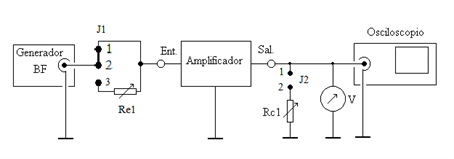
\includegraphics[width=0.9\textwidth]{Imagenes/conexZoLA.png}
    \caption{Conexión del Amplificador de prueba para medir la impedancia de salida}
    \label{fig:conexZoLA}
\end{figure}

El amplificador fue alimentado con una fuente de tensión de 12 V, y la señal de entrada (creada por el generador) tenía una frecuencia de 1 kHz.

Ahora el amplificador se encuentra sin resistencia de carga ($R_{C_1}$), por lo que la tensión que se medirá con el voltímetro y el osciloscopio, será la tensión de salida en vacío. Se procede a variar la tensión de entrada (del generador) hasta justo antes de que la señal de salida se vea recortada (antes de que el amplificador entre en la zona de funcionamiento alineal). Esto se realiza exclusivamente con la finalidad de lograr trabajar con señales más grande para que así sea mas fácil analizarlas y que se vean menos afectadas por el ruido.

La señal de salida $v_s$ máxima que se obtuvo sin recortes fue de 10,2 $V_{pp}$, con una señal de entrada $v_i$ = 3.08 $V_{pp}$.

Sabiendo la tensión de salida en vacío con esa tensión de entrada, se procedió a conectar la carga $R_{C_1}$ (resistor variable), con el jumper $J2$ y se fue variando la resistencia hasta obtener en la salida una señal con la mitad de la amplitud de la señal original. El valor más próximo a este que se obtuvo fue de $v_s'$ = 5,08 $V_{pp}$.

%imagen de la medicion

En esta situación el valor de la impedancia de salida del amplificador es numéricamente igual a la resistencia de carga (debido al tipo de amplificador y la frecuencia en que se hace el ensayo, se puede considerar sin mucho margen de error que la impedancia de salida no tiene parte reactiva considerable), y su valor puede determinarse en forma indirecta midiendo el valor de la resistencia de carga $R_{C_1}$ con un óhmetro. 

Por lo que sin alterar la resistencia, se desconectó el jumper $J2$ para que la medición no se viese afectada por el resto del circuito y se midió la resistencia $R_{C_1}$. En la tabla a continuación se exponen los datos de resistencia recogidos junto con la incertidumbre en la medición (tabla \ref{tab:exp1}).

\subsubsection{Mediciones}

Para la medición de la resistencia se utilizó el multímetro del laboratorio de la marca UNI-T, modelo UT890C, cuyos datos de exactitud, se encuentra en la sección \ref{sec:Información Instrumentos} (Información de Instrumentos), en la tabla \ref{tab:R_UT890C}.

\begin{table}[H]
    \centering
    \scalebox{1}{
    \begin{tabular} {|c|c|c|c|c|}
    %{|m{1.5cm}|m{2.7cm}|m{1cm}|p{1.5cm}|m{2.7cm}|}
   
    \hline
         $f$ & Valor Nominal & $V_s$ & $R_{C_1}=R_o$ & Incertidumbre \\
         
         Frec. Gen. & de $Z_{sal}=R_o$ & en vacío & Para $V_s'=\frac{V_s}{2}$ & medición $R_{C_1}$\\
    \hline
        1 kHz & 50 $\ohm$ & 10.2 $V_{pp}$ & 46.1 $\Omega$ & $\pm$ 0.869 $\Omega$\\
    \hline
        \end{tabular}}
        \def\tablename{Tabla} 
        \caption{Valores esperados y obtenidos}
        \label{tab:exp1}
\end{table}

Afortunadamente, el valor de resistencia obtenido, coincide bastante con el valor esperado para la resistencia de salida. Este es incluso menor, lo que representaría una característica positiva, ya que la impedancia de salida de un amplificador ideal debería ser cero.

\newpage
\label{sec:exp2}
De manera similar a la sección~\ref{sec:exp1}, en este experimento se nos planteo determinar los valores de los componentes planteados en nuestro modelo para una serie de distintos capacitores. Se redujo la resistencia $R_g$ del circuito anterior debido a que el componente resistivo es menor, dejando la resistencia en $R_g=1~k\Omega$. Se modifico la señal de entrada a una señal cuadrada para facilitar las medición. Ya que, como se explico en la sección~\ref{sec:Cap}, la señal en tensión resultante de este planteamiento sera una señal triangular (debido al efecto integrador de corriente del capacitor) sumada a la misma señal cuadrada (debido al efecto de la resistencia interna del capacitor), se podrá discernir y estimar los distintos componentes a través de la medición la señal a bornes del capacitor.

\begin{figure}[H]
    \centering
    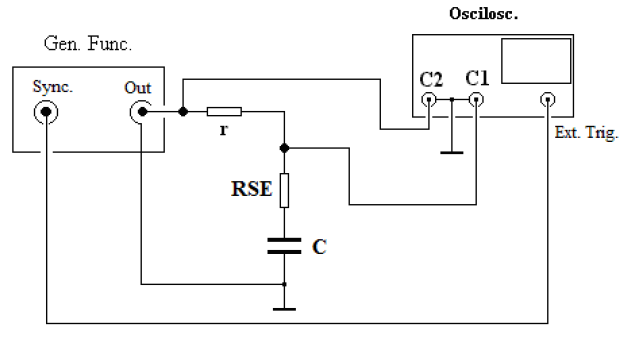
\includegraphics[width=0.7\linewidth]{Imagenes/exp2.png}
    \caption{Circuito experimento 2}
    \label{fig:exp2}
\end{figure}

Según lo anteriormente explicado podemos plantear los siguiente:
\begin{figure}[H]
    \centering
    \begin{minipage}{0.59\textwidth}
        \begin{tikzpicture}[scale=0.65,every node/.style={transform shape}]
\def\res{0.5};%EscalaTemporal señal 1
\def\ind{1};%EscalaTemporal señal 2
\def\scalVa{1};%EscalaVertical señal 1
\def\frec{5};%EscalaVertical señal 2
\def\offseta{0};%Nivel de offset de la señal señal 1
\def\offsetb{};%Nivel de offset de la señal señal 2

%Lineas intermedias grilla
\foreach \x in {-5,-4.8,...,4.8,5}{
    \draw[gray!40,thin,shift={(\x,0)}] (0pt,2pt) -- (0pt,-2pt);
}
\foreach \y in {-4,-3.8,...,3.8,4}{
    \draw[gray!40,thin,shift={(0,\y)}] (2pt,0pt) -- (-2pt,0pt);
}
\foreach \a [evaluate={\y=\a*0.5}] in {-5,-1,1,5}{
    \draw[gray!40,line width=0.7pt,dotted] (-5,\y) -- (5,\y);
}

%Grilla
\draw[thin,gray!40] (-5,-4) grid (5,4);
\node[fill=white,text=gray!40,circle,scale=0.5] at (-5,3) {$100\%$};
\node[fill=white,text=gray!40,circle,scale=0.5] at (-5,2.5) {$90\%$};
\node[fill=white,text=gray!40,circle,scale=0.5] at (-5,-2.5) {$10\%$};
\node[fill=white,text=gray!40,circle,scale=0.5] at (-5,-3) {$0\%$};
\draw[black] (-6,-5) rectangle(6,5);

%Señal 1
\clip (-5,-4) rectangle (5,4);
\foreach [evaluate={\a=\c+2}] \c in{-5,-1,3}{
    \draw[line width=1pt](\c,-2)--(\a,2.5)--(\a,2){};
    \draw[line width=1pt](\a,2)--(\a+2,-2.5)--(\a+2,-2){};
}
\draw[line width=1pt,dashed,stealth-stealth](1,-2.5)--(1,2) node[midway,right]{$v_c$};
\draw[line width=1pt,dashed,stealth-stealth,|-|](-2.8,2)--(-2.8,2.5)node[anchor=north west]{$v_r$};
\end{tikzpicture}
        \label{fig:enter-label}
    \end{minipage}
    \begin{minipage}{0.29\textwidth}
       \begin{circuitikz}[scale=1,every node/.style={transform shape},style=american]
\draw (0,2)to[open,v=$v_i$,o-o](0,-2)--(3,-2)to[capacitor=$C$](3,0)to[R=$r_c$](3,2) (0,2)to[R=$R_g$,i=$i_{(t)}$](3,2);
\draw[line width=0.7pt,dashed] (2.3,-1.8)rectangle(3.3,1.8);
\draw (3.7,0)to[open,v=$v_c$](3.7,-2)  (3.7,2)to[open,v=$v_r$](3.7,0);
\end{circuitikz}

\end{minipage}
\caption{Análisis del circuito equivalente de un capacitor}
\end{figure}
Tomando los valores de los tramos de la señal correspondiente a los distintos componentes, se pude calcular el valor de la resistencia de la siguiente manera:
\begin{equation}
    r_c=\frac{v_r}{i}
\end{equation}

\unsubsubsection{Mediciones}
La señal cuadrada utilizada fue establecida en los siguientes valores: 
\begin{itemize}
    \item $V_{pp}=20~V$
    \item  $F_{rec}=10 ~KHz$
\end{itemize}

Se procedió a medir sobre los puntos establecidos, obteniendo los siguientes datos:
\begin{figure}[H]
    \centering
    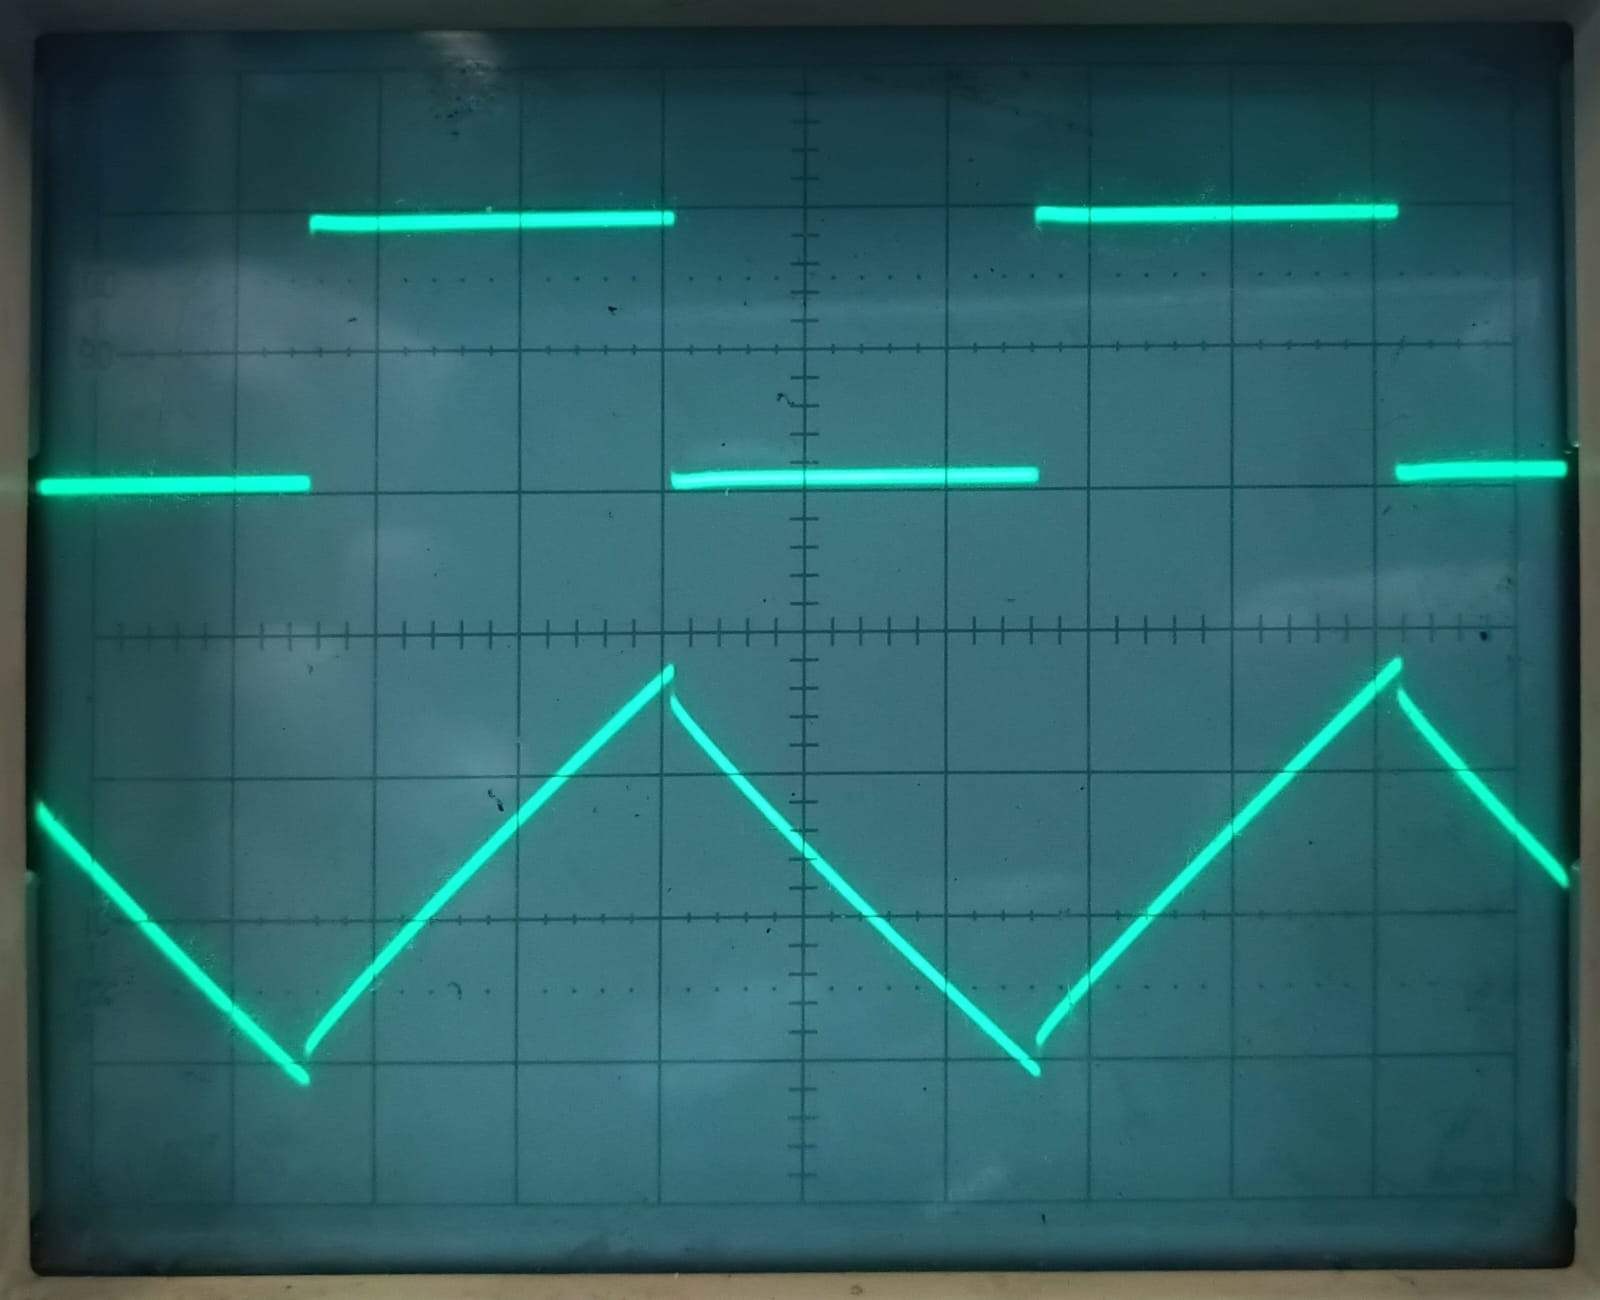
\includegraphics[width=0.6\textwidth]{Imagenes/MedExp2.jpeg}
    \caption{Mediciones de la señal de salida vs entrada del experimento 2}

\end{figure}
\begin{table}[H]
    \centering
    \begin{tabular}{|c|c|c|c|}
    \hline
        $f$ & \multicolumn{3}{c|}{$10~kHz$}\\
    \hline
        $C_{nom}$ & $1~\mu F$ & $2.2~\mu F$ & $4.7~\mu F$ \\ 
    \hline
        $r$ & \multicolumn{3}{c|}{$1~k\Omega$}\\
    \hline
        $e_{pp}~(Canal~2)[V]$ & 20 & 20 & 20\\
    %\hline
        $I=\cfrac{e_{pp}}{r} ~[mA]$ & 18.5 & 18.5 & 18.5 \\
    %\hline    
        $e_R~[mV]$ & 36 & 149.85 & 50 \\
    %\hline    
        $RSE = \cfrac{e_R}{I} ~[\Omega]$ & 1.94 & 7.3 & 2.7 \\
    \hline    
    
        \end{tabular}
        \def\tablename{Tabla} 
        \caption{Tabla de parámetros para distintos capacitores}
        \label{tab:exp2}
\end{table}

\unsubsubsection{Comprobación}
Utilizando un medidor RLC se comprobaron los valores nominales de los 3 capacitores utilizados:

\begin{figure}[H]
\centering
    \begin{minipage}{0.29\textwidth}
    \centering
    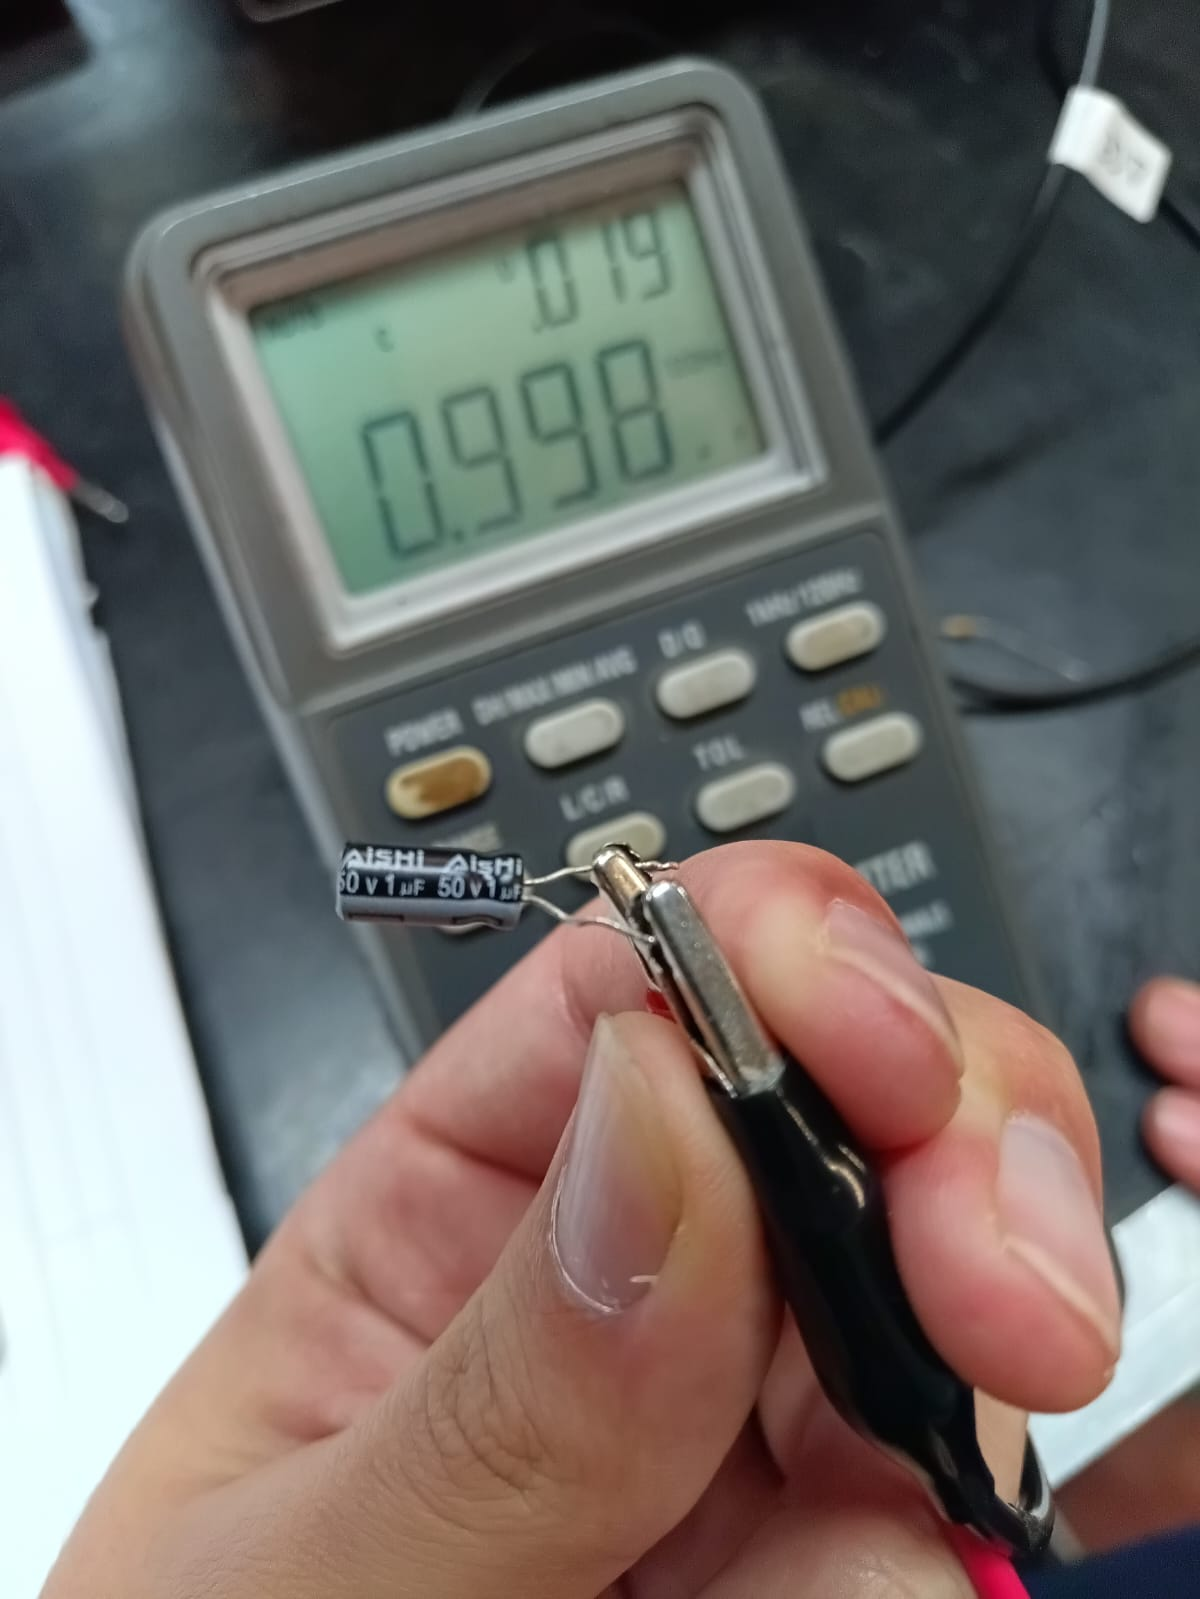
\includegraphics[width=\textwidth,trim={0cm 10cm 0cm 0cm},clip]{Imagenes/MedCap3Exp2.jpeg}
    \caption*{$C=1~\mu F$}
    \end{minipage}
    \hspace*{\fill}
    \begin{minipage}{0.29\textwidth}
    \centering
    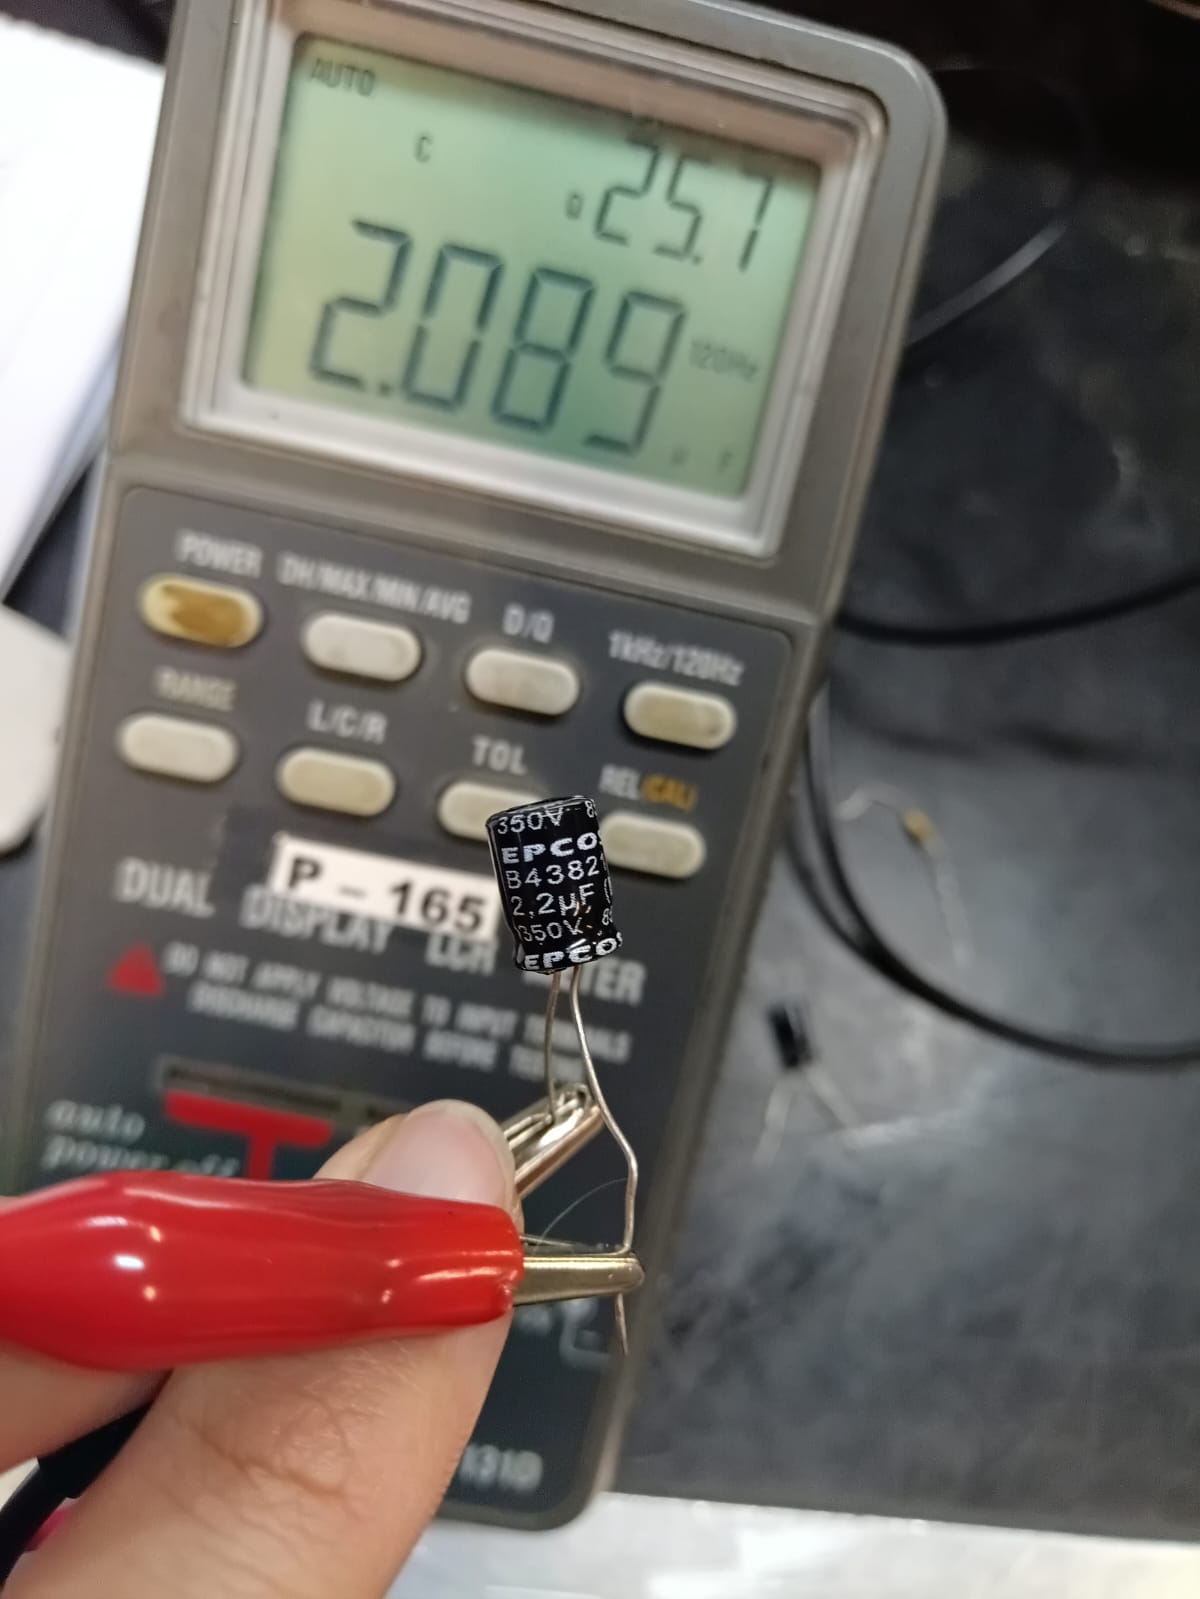
\includegraphics[width=\textwidth,trim={0cm 10cm 0cm 0cm},clip]{Imagenes/MedCap1Exp2.jpeg}
    \caption*{$C=2.2~\mu F$}
    \end{minipage}
    \hspace*{\fill}
    \begin{minipage}{0.29\textwidth}
    \centering
    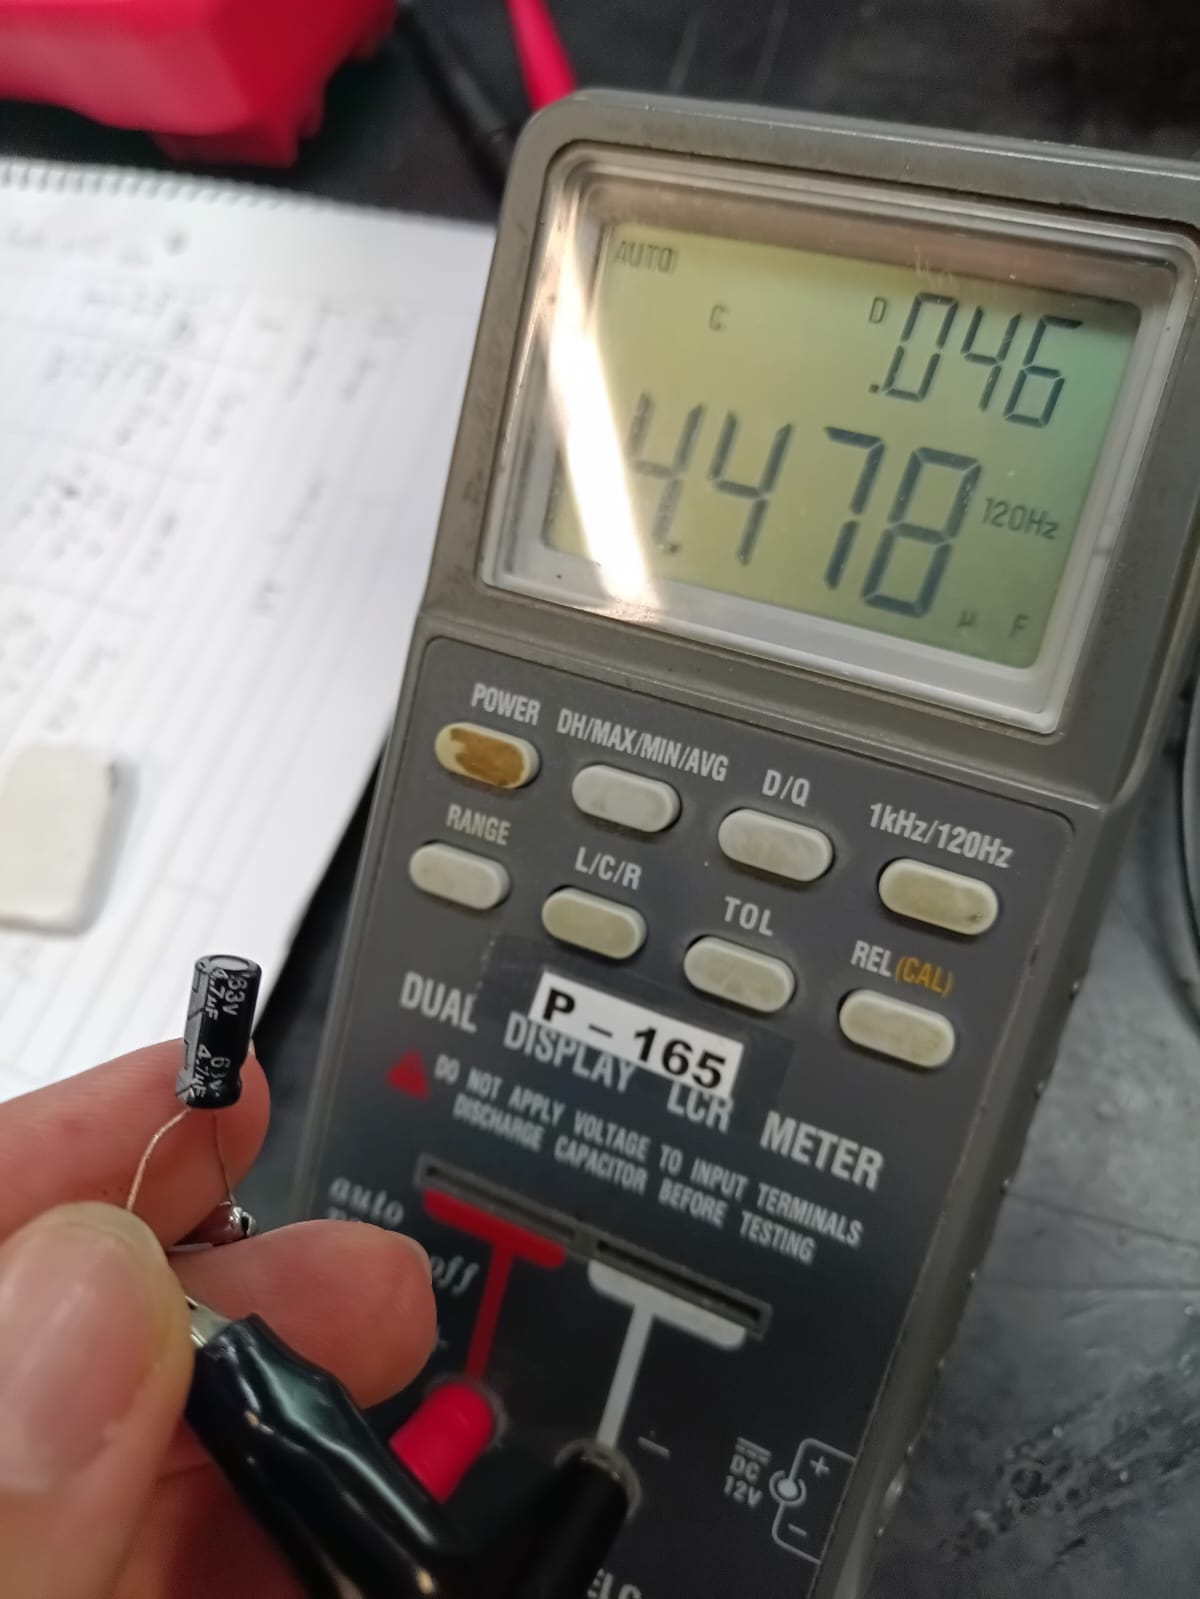
\includegraphics[width=\textwidth,trim={0cm 10cm 0cm 0cm},clip]{Imagenes/MedCap2Exp2.jpeg}
    \caption*{$C=4.7~\mu F$}
    \end{minipage}
    \caption{Mediciones de los capacitores del experimento 2}
\end{figure}


\newpage
\section{Conclusión}


Con el presente trabajo se pudo aprender a como medir las impedancias y el ancho de banda de los amplificadores correctamente, parámetros muy importante para nuestra carrera. Además de medir lo efectos que tiene sobre estos parámetros la realimentación negativa.
Se pudo observar que, la realimentación negativa, aumenta el ancho de banda del amplificador a costa de reducir la ganancia. La realimentación negativa, además de tener un efecto sobre la respuesta en frecuencia, afecta las impedancias tanto de entrada como de salida. La impedancia de entrada aumentara, incrementando la ganancia en potencia del amplificador. Recordando la ecuación \ref{eq:Exp4PotZ},$P_{dB}=GV_{dB}-10\log{\frac{Z_L}{Z_e}}$ el efecto del segundo termino (correspondiente a las impedancias) tendrá un mayor efecto, aumentando la ganancia. Claro esto solo si tenemos en cuenta el efecto que tienen las resistencias y despreciando la perdida de ganancia en tensión. En cuanto a la transferencia de potencia, la disminución de la impedancia de salida no involucra una mayor potencia sobre la carga. Ahora, en el caso de la impedancia de entrada es de esperar que aumente la resistencia al ser una realimentación del tipo comparación de tensiones en serie.

Se aprendió a utilizar la escala de decibelios en el multimetro y como calibrarlo.
El usar un multimetro con escala en decibelios te da muchas ventajas que simplifican la experimentación, algunas de estas son:
\begin{itemize}
    \item Facilidad en el calculo, ya que la ganancia se obtiene realizando directamente la diferencia entre los valores de entrada y de salida, permitiendo observar fácilmente si nuestro amplificador magnifica, atenúa o no amplifica la señal de entrada.
    \item Permite visualizar de manera cómoda la variación de la ganancia en función de factores que poseen un amplio rango de variación.
    \item Al medir algún parámetro (potencia o tensión), el uso de escalas en decibeles permite visualizar de manera rápida y directa la magnitud medida. 
    \item El decibel se calcula en una escala logarítmica que permite la especificación del rendimiento a través de un amplio rango de voltaje/potencia.
\end{itemize}

En caso de que se cambie la escala,(respecto a el rango de $3V$)de un multimetro analógico al medir en decibelios, se debe aplicar un factor de corrección para las mediciones:
\begin{equation}
    dBu=dBu'+\log{\frac{Vr_1}{Vr_0}}
\end{equation}
Siendo $dBu'$ el valor medido por el multimetro, $Vr_0$ el valor de la escala inicial (en nuestro caso $3V$) y $Vr_1$ el valor de la nueva escala.





\vspace{3cm}
\section{Bibliografía}
\begin{itemize}
   \item \url{https://slideplayer.es/slide/16695348/}
   \item \url{https://www.tel.uva.es/personales/lib/osciloscopio.html#:~:text=Con%20este%20mismo%20pulsador%2C%20cada,la%20parte%20ascendente%20o%20descendente.}
   \item \url{https://www.fceia.unr.edu.ar/eca1/files/teorias/osciloscopio.pdf}
    \item \url{https://www.manualslib.com/manual/1574416/Bk-Precision-2120c.html}
\end{itemize}


\end{document}